\documentclass{beamer}
\usetheme{Madrid}
\usecolortheme{default}
\usepackage{listings}
\usepackage{xcolor}
\usepackage{booktabs}
\definecolor{codebg}{rgb}{0.96,0.96,0.96}
\lstset{basicstyle=\ttfamily\scriptsize, backgroundcolor=\color{codebg},
  breaklines=true, columns=fullflexible, frame=single, framesep=2pt}

\title{Sampling and Per-Precision Histograms with nixnan}
\subtitle{An Experiment on \texttt{rd\_nixnan.cu}}
\author{ganesh@cs.utah.edu}
\date{\today}

\begin{document}

\frame{\titlepage}

% ------------------------------------------------------------------
\begin{frame}{The Example, at a Glance}
\texttt{rd\_nixnan.cu}: a 1D reaction-diffusion PDE
$\partial u/\partial t = D\,\partial^2 u/\partial x^2 + \lambda u$,
explicit FTCS, 101-point grid, 1600 steps --- the \emph{same} kernel
implemented once each in FP16, BF16, FP32, FP64.

\vspace{0.5cm}
\textbf{How precision-sensitive is this example?}
\begin{itemize}
  \item The reaction term grows every value by ${\sim}1.05\times$ per step,
    \emph{regardless of format} --- so the only thing that differs between
    formats is how much exponent range each one has before it overflows.
  \item FP16's 5-bit exponent runs out at step 300; BF16/FP32/FP64's
    wider exponents are all still finite at step 1600 --- same algorithm,
    same input, one format fails and three don't.
\end{itemize}
\end{frame}

% ------------------------------------------------------------------
\begin{frame}[fragile]{Concept 1: Sampling --- The Mechanism}
Every run here uses \texttt{nixnan.so} directly (``straight nixnan''), no
wrapper:
\begin{lstlisting}[language=bash]
LD_PRELOAD=<path>/nixnan.so [ENV_VARS...] ./rd_nixnan
\end{lstlisting}
\texttt{SAMPLING=N} instruments only every $N$th launch of a repeated
kernel --- a knob trading overhead for observation completeness.

\vspace{0.3cm}
\textbf{Verified before trusting it:} an older comment in this repo claims
\emph{``SAMPLING is a no-op.''} We re-tested directly (\texttt{SAMPLING=1}
vs.\ \texttt{SAMPLING=100000}): exception counts dropped to exactly zero at
the high value. \textbf{Confirmed fixed} in the current build.
\end{frame}

% ------------------------------------------------------------------
\begin{frame}[fragile]{Concept 1: Every Call vs.\ Once in 8}
FP16 exception counts (the only format that overflows here):
\begin{center}
\begin{tabular}{lrr}
\toprule
 & NaN (unique / repeats) & Infinity (unique / repeats) \\
\midrule
\texttt{SAMPLING=1} (every call) & 22 / 60{,}534 & 22 / 639 \\
\texttt{SAMPLING=8} & 22 / 7{,}524 & 17 / 66 \\
\bottomrule
\end{tabular}
\end{center}
\vspace{0.3cm}
Repeats drop ${\sim}8\times$, as expected. But \textbf{5 distinct Infinity
sites vanish entirely} (22 $\to$ 17) --- coarse sampling doesn't just
under-count, it can miss whole bugs.
\end{frame}

% ------------------------------------------------------------------
\begin{frame}[fragile]{Concept 1: An Exponentially Decaying Schedule}
\texttt{SAMPLING} is fixed for a whole process run, so a decaying rate is
built as a sequence of short runs (\texttt{sampling\_schedule.json}):
step 4 times at spacing 1 $\to$ double to 2 $\to$ 4 $\to$ 8 $\to$ \textbf{reset}.
\begin{center}
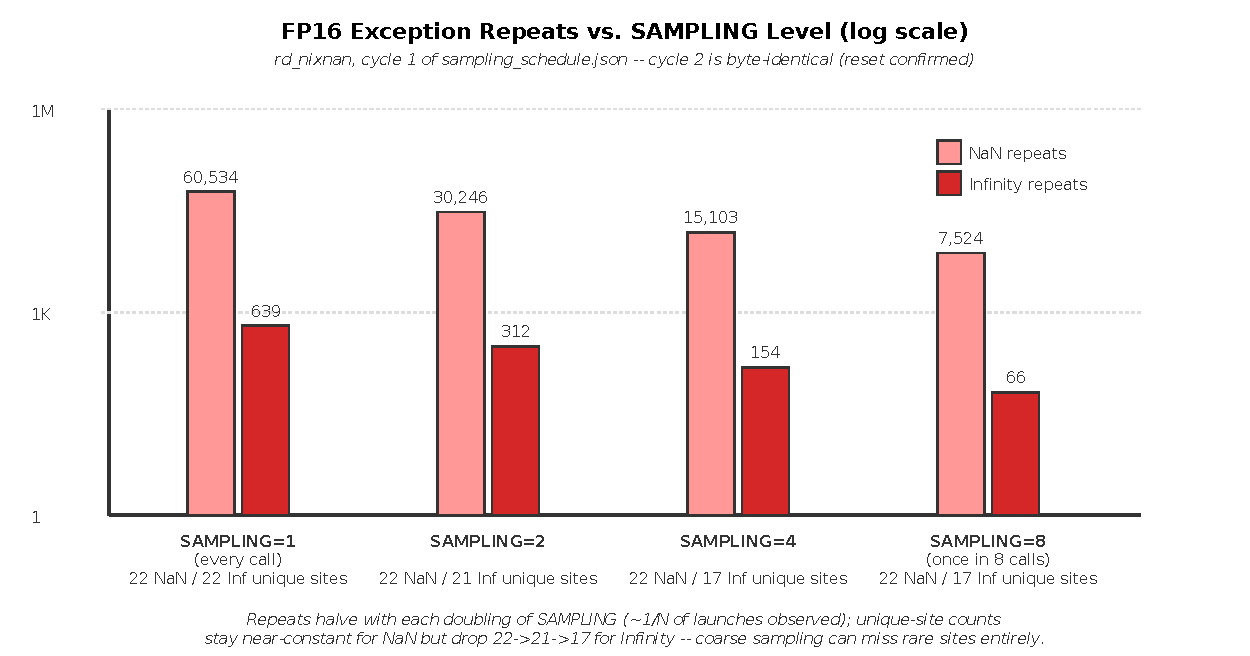
\includegraphics[width=0.85\textwidth]{../viz/sampling_decay.pdf}
\end{center}
Every snap at a level is byte-identical; \textbf{cycle 2 exactly reproduces
cycle 1} --- the reset is provably clean.
\end{frame}

% ------------------------------------------------------------------
\begin{frame}[fragile]{Concept 2: Histograms per Precision --- The Mechanism}
\texttt{HISTOGRAM=1} tracks the exponent of every instrumented FP value,
independent of exception checking:
\begin{lstlisting}[language=bash]
HISTOGRAM=1 LD_PRELOAD=nixnan.so ./rd_nixnan
\end{lstlisting}
At exit, nixnan reports the $[\min,\max]$ exponent \emph{actually observed}
for each format --- one number per precision bucket, no per-value log
needed.
\end{frame}

% ------------------------------------------------------------------
\begin{frame}{Concept 2: Results --- Which Format Actually Failed}
\begin{center}
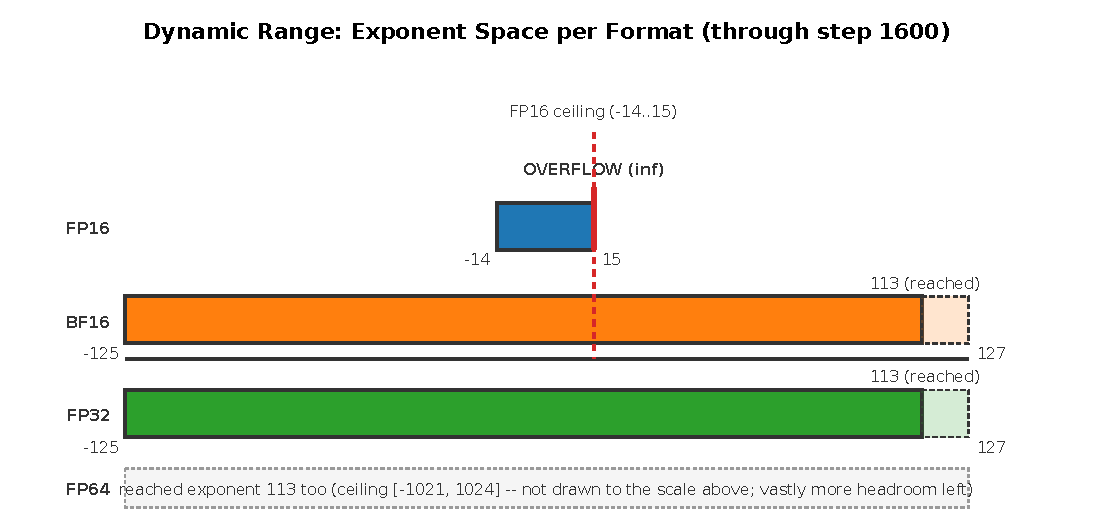
\includegraphics[width=0.85\textwidth]{../viz/exponent_ranges_per_precision.pdf}
\end{center}
\texttt{f16} alone reports \texttt{inf}. \texttt{bf16}/\texttt{f32}/\texttt{f64}
all reach the \emph{identical} exponent, 113 --- same trajectory, different
ceilings, only one ceiling reached.
\end{frame}

% ------------------------------------------------------------------
\begin{frame}{What nixnan Made Visible Here}
\begin{enumerate}
  \item \textbf{Sampling trades overhead for completeness}, not just
    verbosity --- coarse sampling can drop entire exception sites, not
    only reduce their reported repeat count.
  \item \textbf{A schedule can be built around a static env var} via
    orchestration, and --- because the program is deterministic --- that
    schedule's reset is independently verifiable.
  \item \textbf{Per-format exponent histograms turn ``FP16 probably fails''
    into a specific, quantified claim}: FP16 alone overflows; the other
    three formats are proven to share one common growth trajectory up to
    a shared checkpoint exponent.
\end{enumerate}
\vspace{0.3cm}
\textit{Bonus: re-verifying SAMPLING here also caught that a previously
documented nixnan regression has since been fixed.}
\end{frame}

\end{document}
